\documentclass[a4paper,10pt]{report}
\usepackage[polish]{babel}
\usepackage[utf8]{inputenc}
\usepackage[T1]{fontenc}
\usepackage{times}
\usepackage{graphicx}
\usepackage{anysize}
\usepackage{longtable}
\usepackage{array}

%\marginsize{left}{right}{top}{bottom}
\marginsize{5cm}{5cm}{5cm}{5cm}

\begin{document}


Nauka zajmująca się badaniem i~poznawaniem budowy organizmów ptaków oraz ich życia nosi nazwę \emph{ornitologii} i~jest częścią \emph{zoologii}. Do tej dyscypliny naukowej należy morfologia, tj. nauka o~wyglądzie i~budowie zewnętrznej i~wewnętrznej ptaka, biologia -- nauka o~wszelkich przejawach ich życia fizycznego: ekologia, nauka o~wymaganych przez dany gatunek warunkach środowiskowych oraz etologia -- nauka o~zwyczajach i~sposobie zachowania się poszczególnych gatunków. W~zakres wiedzy ornitologicznej wchodzi również systematyka zoologiczna, polegająca na podziale wszystkich ptaków na grupy systematyczne (gromada, rząd, rodzina, rodzaj, gatunek) według bliższego lub dalszego pokrewieństwa. 

Niezależnie od systematyki przyjęto tutaj podział wszystkich ptaków na trzy grupy według ich użyteczności gospodarczej: ptaki łowne, które w~okresie lęgów znajdują się pod tzw. ochroną okresową, ptaki objęte całoroczną ochroną, zwaną gatunkową, ptaki, które w~ciągu całego roku w~ogóle nie podlegają ochronie.


Stosunkowo nieliczny gatunek osiadły i~zalatujący. Żyje w~starych lasach, w~pobliżu których znajdują się skaliste zbocza, poręby, łąki, miejsca rzadko odwiedzane. Gatunek monogamiczny łączący się w~pary prawdopodobnie na całe życie. Okres gniazdowania: luty-kwiecień. Gniazda buduje z gałązek, umieszcza na drzewie lub na skale, samica wyściela je miękkim materiałem. Składa 4-6 zielonkawych jaj kształtu jajowatego z~brązowymi plamami. Wysiaduje wyłącznie samica przez około 3~tygodnie; samiec ją w~tym czasie żywi. Pisklęta są gniazdownikami, karmione przez obydwoje rodziców około 40 dni. 

\begin{figure}[t]
\centerline{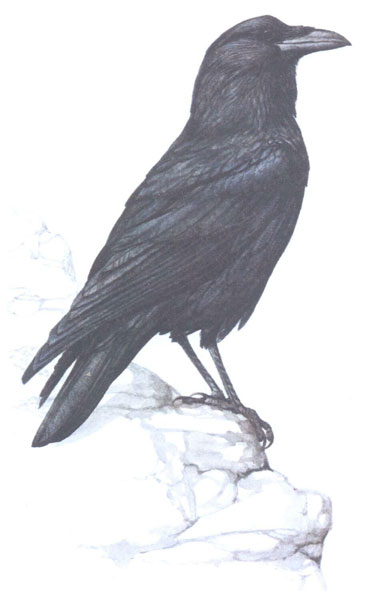
\includegraphics[scale=0.2]{kruk}}
\caption{Kruk1}
\end{figure}

\begin{figure}[b]
\centerline{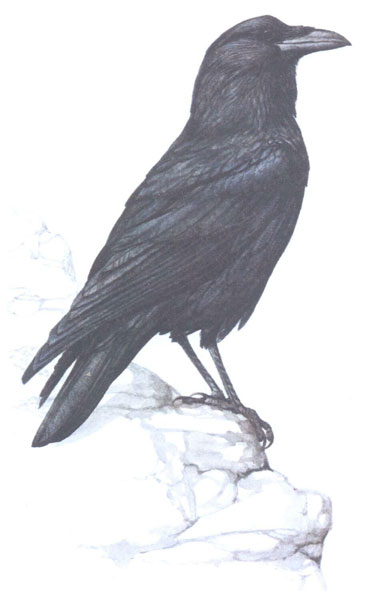
\includegraphics[scale=0.2]{kruk}}
\caption{Kruk2}
\end{figure}

\begin{figure}[h]
\centerline{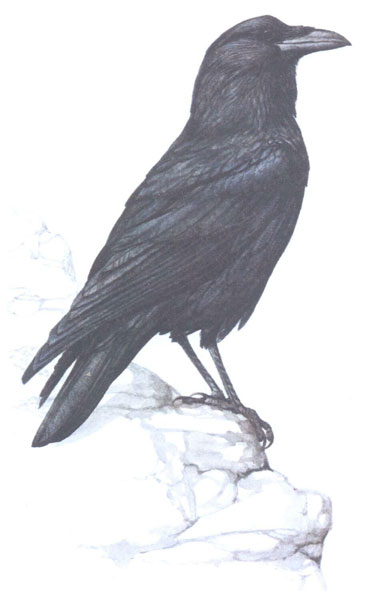
\includegraphics[scale=0.2]{kruk}}
\caption{Kruk3}
\end{figure}

Pospolity gatunek osiadły i~zalatujący. Przebywa najchętniej na terenach nizinnych w~zagajnikach, alejach, parkach. Na terenach pagórkowatych występuje rzadko. W zimie stada gawronów pojawiają się w~wielkich ilościach na polach oraz w~osiedlach ludzkich, przeważnie są to osobniki z~krajów położonych na północny wschód od Polski. Gnieździ się w~koloniach na skrajach lasów, w~zagajnikach i~dużych parkach. Gniazdo umiejscawia na wysokich drzewach z~dobrze rozwiniętą koroną. Jest ono dość niestarannie zbudowane z~suchych gałązek trawy i~suchych korzonków, wewnątrz wysłane sierścią. Gatunek monogamiczny. Okres gniazdowania: marzec-kwiecień. Samica znosi 3-5 jasnych, niebieskozielonych jaj, kształtu jajowatego, gęsto usianych żółtawymi i~brązowymi plamkami. Jaja wysiaduje samica przez 18-19 dni. Pisklęta są gniazdownikami. Rodzice karmią młode przez 28-30 dni. 


\begin{longtable}{|c|c|c|c|c|c|c|c|c|c|}
\caption{Warunki terenowe}
\label{tab:warunkiTerenowe}\\
\cline{2-10} 
\multicolumn{1}{l|}{} & \multicolumn{9}{|c|}{Zwrotnice} \\ \hline
{Przebiegi} & 3/4 & 5 & 6 & 7/8 & 15/16 & 17 & 18 & 19/20 & 21/22 \\ \hline
\endfirsthead
\cline{2-10} 
\multicolumn{1}{l|}{} & \multicolumn{9}{|c|}{Zwrotnice} \\ \hline
{Przebiegi} & 3/4 & 5 & 6 & 7/8 & 15/16 & 17 & 18 & 19/20 & 21/22 \\ \hline
\endhead
\multicolumn{10}{|c|}{Stopka tabeli} \\ \hline
\endfoot
\multicolumn{10}{|c|}{Stopka na ostatniej stronie} \\ \hline
\endlastfoot
B1 & + & + &  &  &  &  &  &  &  \\ \hline
B2 & -- &  & + & o+ &  &  &  &  &  \\ \hline
B3 & + & -- &  &  &  &  &  &  &  \\ \hline
B4 & -- &  & -- & + & o+ &  &  &  &  \\ \hline
R2 &  &  &  & o+ & o+ & + &  & + & + \\ \hline
R4 &  &  &  & o+ & + & -- &  & + & + \\ \hline
F2W & + &  & + & o+ &  &  &  &  &  \\ \hline
G2W & + &  & -- & + &  &  &  &  &  \\ \hline
K1D &  &  &  &  & + & -- &  & -- & + \\ \hline
L1D &  &  &  &  & o+ & + &  & -- & + \\ \hline
M1D &  &  &  &  &  &  & + & + & + \\ \hline
N1D &  &  &  &  &  &  & -- & + & + \\ \hline
B1 & + & + &  &  &  &  &  &  &  \\ \hline
B2 & -- &  & + & o+ &  &  &  &  &  \\ \hline
B3 & + & -- &  &  &  &  &  &  &  \\ \hline
B4 & -- &  & -- & + & o+ &  &  &  &  \\ \hline
R2 &  &  &  & o+ & o+ & + &  & + & + \\ \hline
R4 &  &  &  & o+ & + & -- &  & + & + \\ \hline
F2W & + &  & + & o+ &  &  &  &  &  \\ \hline
G2W & + &  & -- & + &  &  &  &  &  \\ \hline
K1D &  &  &  &  & + & -- &  & -- & + \\ \hline
L1D &  &  &  &  & o+ & + &  & -- & + \\ \hline
M1D &  &  &  &  &  &  & + & + & + \\ \hline
N1D &  &  &  &  &  &  & -- & + & + \\ \hline
B1 & + & + &  &  &  &  &  &  &  \\ \hline
B2 & -- &  & + & o+ &  &  &  &  &  \\ \hline
B3 & + & -- &  &  &  &  &  &  &  \\ \hline
B4 & -- &  & -- & + & o+ &  &  &  &  \\ \hline
R2 &  &  &  & o+ & o+ & + &  & + & + \\ \hline
R4 &  &  &  & o+ & + & -- &  & + & + \\ \hline
F2W & + &  & + & o+ &  &  &  &  &  \\ \hline
G2W & + &  & -- & + &  &  &  &  &  \\ \hline
K1D &  &  &  &  & + & -- &  & -- & + \\ \hline
L1D &  &  &  &  & o+ & + &  & -- & + \\ \hline
M1D &  &  &  &  &  &  & + & + & + \\ \hline
N1D &  &  &  &  &  &  & -- & + & + \\ \hline
B1 & + & + &  &  &  &  &  &  &  \\ \hline
B2 & -- &  & + & o+ &  &  &  &  &  \\ \hline
B3 & + & -- &  &  &  &  &  &  &  \\ \hline
B4 & -- &  & -- & + & o+ &  &  &  &  \\ \hline
R2 &  &  &  & o+ & o+ & + &  & + & + \\ \hline
R4 &  &  &  & o+ & + & -- &  & + & + \\ \hline
F2W & + &  & + & o+ &  &  &  &  &  \\ \hline
G2W & + &  & -- & + &  &  &  &  &  \\ \hline
K1D &  &  &  &  & + & -- &  & -- & + \\ \hline
L1D &  &  &  &  & o+ & + &  & -- & + \\ \hline
M1D &  &  &  &  &  &  & + & + & + \\ \hline
N1D &  &  &  &  &  &  & -- & + & + \\ \hline
B1 & + & + &  &  &  &  &  &  &  \\ \hline
B2 & -- &  & + & o+ &  &  &  &  &  \\ \hline
B3 & + & -- &  &  &  &  &  &  &  \\ \hline
B4 & -- &  & -- & + & o+ &  &  &  &  \\ \hline
R2 &  &  &  & o+ & o+ & + &  & + & + \\ \hline
R4 &  &  &  & o+ & + & -- &  & + & + \\ \hline
F2W & + &  & + & o+ &  &  &  &  &  \\ \hline
G2W & + &  & -- & + &  &  &  &  &  \\ \hline
K1D &  &  &  &  & + & -- &  & -- & + \\ \hline
L1D &  &  &  &  & o+ & + &  & -- & + \\ \hline
M1D &  &  &  &  &  &  & + & + & + \\ \hline
N1D &  &  &  &  &  &  & -- & + & + \\ \hline
\end{longtable}

Pospolity ptak lęgowy i~przelotny. Przylatuje w~połowie kwietnia, odlatuje od sierpnia do września, czasem dopiero w~październiku. Żyje w~mniejszych miastach i~na wsiach, unika większych miast. Gnieździ się w~budynkach, najchętniej w~stajniach i~oborach, pod dachem. Gniazdo ma kształt miskowaty, zbudowane jest z~gliny i~źdźbeł trawy zmieszanych ze śliną. Wnętrze wysłane jest pierzem i~sierścią. Gatunek monogamiczny. Gniazduje dwa razy w roku -- w~maju i~w~czerwcu. Znosi 4-6 białych jaj kształtu jajowatego z~fioletowoszarymi i~brązowoczerwonymi plamkami. Wysiadywanie trwa 14-16 dni. Pisklęta są rzekomymi gniazdownikami, legną się okryte białawym puchem. Wykarmianie piskląt trwa około 24 dni. 


\begin{figure}[ht]
\centerline{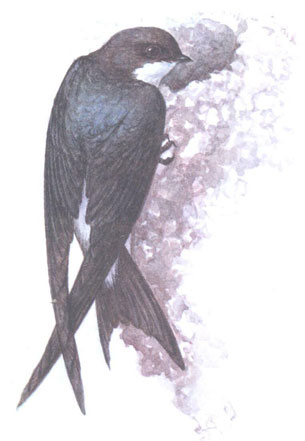
\includegraphics[scale=0.2]{jaskolka-oknowka}}
\caption{Jaskółka oknówka}
\label{fig:jaskolkaoknowka}
\end{figure}

Liczny gatunek lęgowy i~przelotny. Przylatuje w~kwietniu, odlatuje we wrześniu. Przebywa w~miejscach, w~których żyje również jaskółka dymówka. Gniazdo buduje pod dachami budynków, rzadziej gnieździ się wewnątrz budynku. Gniazdo jest ulepione z~gliny zmieszanej z~błotem i~śliną, w~kształcie ćwierć kuli przyczepionej pod okapem dachu do ściany. Wewnątrz wysłane jest pierzem i~sierścią. Gatunek monogamiczny. Gniazduje dwa razy w~ciągu roku. Znosi 4-5 czystobiałych jaj, kształtu jajowatego. Wysiaduje samiczka i~samiec przez około dwa tygodnie. Pisklęta karmione przez 21-23 dni, są rzekomymi gniazdownikami, lęgną się okryte białawym puchem. Na rysunku~\ref{fig:jaskolkaoknowka} pokazano jaskółkę oknówkę.

\begin{table}
\centerline{
\begin{tabular}{|p{8mm}|p{8mm}|p{8mm}|}
\hline
x y z x y z x y z x y z x y z & x y z x y z x y z & 1 1 1 1 1 \\\hline
\end{tabular}}
\end{table}

\begin{table}
\centerline{
\begin{tabular}{|m{8mm}|m{8mm}|m{8mm}|}
\hline
x y z x y z x y z x y z x y z & x y z x y z x y z & 1 1 1 1 1 \\\hline
\end{tabular}}
\end{table}

\begin{table}
\centerline{
\begin{tabular}{|b{8mm}|b{8mm}|b{8mm}|}
\hline
x y z x y z x y z x y z x y z & x y z x y z x y z & 1 1 1 1 1 \\\hline
\end{tabular}}
\end{table}









\end{document}
